%%
%% Copyright 2007, 2008, 2009 Elsevier Ltd
%%
%% This file is part of the 'Elsarticle Bundle'.
%% ---------------------------------------------
%%
%% It may be distributed under the conditions of the LaTeX Project Public
%% License, either version 1.2 of this license or (at your option) any
%% later version.  The latest version of this license is in
%%    http://www.latex-project.org/lppl.txt
%% and version 1.2 or later is part of all distributions of LaTeX
%% version 1999/12/01 or later.
%%
%% The list of all files belonging to the 'Elsarticle Bundle' is
%% given in the file `manifest.txt'.
%%

%% Template article for Elsevier's document class `elsarticle'
%% with numbered style bibliographic references
%% SP 2008/03/01
%%
%%
%%
%% $Id: elsarticle-template-num.tex 4 2009-10-24 08:22:58Z rishi $
%%
%%
\documentclass[preprint,12pt,3p]{elsarticle}

%% Use the option review to obtain double line spacing
%% \documentclass[preprint,review,12pt]{elsarticle}

%% Use the options 1p,twocolumn; 3p; 3p,twocolumn; 5p; or 5p,twocolumn
%% for a journal layout:
%% \documentclass[final,1p,times]{elsarticle}
%% \documentclass[final,1p,times,twocolumn]{elsarticle}
%% \documentclass[final,3p,times]{elsarticle}
%% \documentclass[final,3p,times,twocolumn]{elsarticle}
%% \documentclass[final,5p,times]{elsarticle}
%% \documentclass[final,5p,times,twocolumn]{elsarticle}

%% if you use PostScript figures in your article
%% use the graphics package for simple commands
%% \usepackage{graphics}
%% or use the graphicx package for more complicated commands
%% \usepackage{graphicx}
%% or use the epsfig package if you prefer to use the old commands
%% \usepackage{epsfig}

%% The amssymb package provides various useful mathematical symbols
\usepackage{amssymb}
%% The amsthm package provides extended theorem environments
%% \usepackage{amsthm}

%% The lineno packages adds line numbers. Start line numbering with
%% \begin{linenumbers}, end it with \end{linenumbers}. Or switch it on
%% for the whole article with \linenumbers after \end{frontmatter}.
\usepackage{lineno}

%% natbib.sty is loaded by default. However, natbib options can be
%% provided with \biboptions{...} command. Following options are
%% valid:

%%   round  -  round parentheses are used (default)
%%   square -  square brackets are used   [option]
%%   curly  -  curly braces are used      {option}
%%   angle  -  angle brackets are used    <option>
%%   semicolon  -  multiple citations separated by semi-colon
%%   colon  - same as semicolon, an earlier confusion
%%   comma  -  separated by comma
%%   numbers-  selects numerical citations
%%   super  -  numerical citations as superscripts
%%   sort   -  sorts multiple citations according to order in ref. list
%%   sort&compress   -  like sort, but also compresses numerical citations
%%   compress - compresses without sorting
%%
%% \biboptions{comma,round}

% \biboptions{}


\journal{ECE Prospectus}

\begin{document}

\begin{frontmatter}

\title{Adopting Essence Kernel, Understanding Agile Iterative Software Development}

\author{Todd Sedano}
\ead{todd.sedano@sv.cmu.edu}

\author{C\'ecile P\'eraire}
\ead{cecile.peraire@sv.cmu.edu}

\address{Carnegie Mellon University}
\address{Silicon Valley Campus}
\address{Moffett Field, CA 94035, USA}


\begin{abstract}
The Software Engineering Method and Theory (SEMAT) community created the Essence kernel as a unifying framework for describing and analyzing software engineering endeavors. The Essence kernel is based upon human experience and judgment, not empirical data. 

Background: At Carnegie Mellon University in Silicon Valley, we have collected data from masters of science in software engineering students as they complete a team-based project course as their capstone or practicum project using the Essence kernel. Each week, the team recorded their progress in an Essence Reflection meeting. This data serves as training data for evaluating the Essence kernel and alternative candidate kernels.

Objective: To adapt the Essence Kernel for use at Pivotal by providing a kernel extension to match Pivotal's engineering practices.

Method: Observe several software development projects at Pivotal. Interview several engineers. Iterative research incorporating feedback from several engineers. Review the proposed Pivotal Extension with software engineers and product owners. 

Expected Results: A modified kernel or kernel extension grounded in empirical data that supports interactive software development. 

Limitations: While the results are highly relevant to Pivotal, the outcomes may not be transferable to other software development organizations in different domains or geographies.

Conclusion: The original Essence kernel is method agnostic and does not directly support iterative development. During Essence Reflection Meetings, student teams using the Essence Kernel find value during project inception and start-up and find less value during an iterative construction phase. Since most of agile software development occurs via interactive construction adapting Essence kernel would increase its value to software development teams.

\end{abstract}

\begin{keyword}
%% keywords here, in the form: keyword \sep keyword
Essence Kernel \sep Empirical Research
%% MSC codes here, in the form: \MSC code \sep code
%% or \MSC[2008] code \sep code (2000 is the default)
\end{keyword}

\end{frontmatter}

%%
%% Start line numbering here if you want
%%
\linenumbers

%% main text
\section{Background}
The SEMAT community created Essence as a universal framework for any software engineering project. At the core of Essence is a ``kernel of widely-agreed elements'' ~\cite{JacobsonQueue}. This general kernel can theoretically support any kind of software endeavor. A software project can define its software processes by using the general kernel, extending the kernel, or defining additional practices on top of the kernel.

The Essence kernel is composed of a set of alphas, alpha states, and alpha state checklist items. The Essence kernel defines different characteristics or dimensions of a software project as an ``alpha.'' The seven alphas are \textbf{Stakeholders}, \textbf{Opportunity}, \textbf{Requirements}, \textbf{Software System}, \textbf{Team}, \textbf{Way of Working}, and \textbf{Work}. Essence decomposes each of these alphas into a set of states that represent a simple linear state machine as shown in Figure \ref{StateMachine}. For example, the \textbf{Requirements} alpha advances through the states \textit{Conceived}, \textit{Bounded}, \textit{Coherent}, \textit{Acceptable}, \textit{Addressed}, and \textit{Fulfilled.} Each state has a checklist or set of goals. To achieve a state, the project must satisfy every checklist item for that state. \cite{OMGStandard} 
 
\begin{figure}[h]\vspace*{4pt}
\centerline{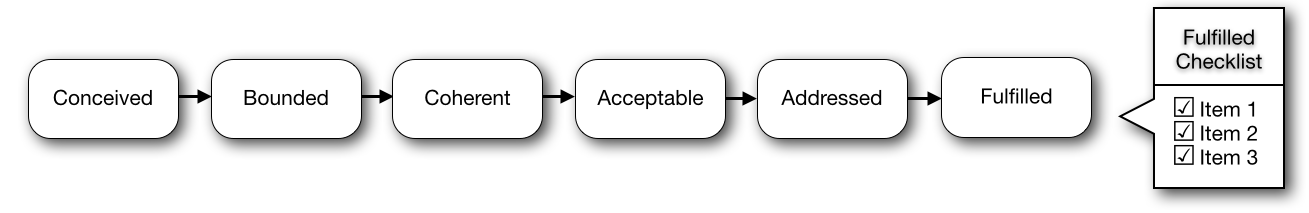
\includegraphics[width=5.4in]{kernel_images/StateMachineRequirements}}
\caption{Kernel's linear state machine for Requirements alpha (with Fulfilled Checklist)}\vspace*{-6pt}\label{StateMachine}
\end{figure}

When the SEMAT community created the Essence kernel, they relied upon human experience and judgment to select the alphas, states, and checklists. Essence is not grounded by empirical data. There might be other possible groupings of checklist items that are more effective which we might not normally consider because they do not match our preconceived notions of structure and order.

I performed a field study \cite{ICSE2014} to understand the value project teams receive from following the SEMAT Essence’s monitoring and steering approach provided by the Essence kernel alphas and their states. The study involved seven teams of software engineering master students with no prior knowledge of Essence. The study showed that the approach provides student teams with a simple, lightweight, non- prescriptive and method-agnostic way to examine their projects holistically, structure team reflections, manage risks, monitor progress and steer their projects. Compared to the ten previous years, the faculty in charge of the practicum course noted that there was “much better early project organization with a lot less floundering.” Indeed, the approach enables students to learn to steer projects effectively by addressing the various dimensions of software engineering.

The study also highlighted that the monitoring and steering mechanisms are most effective during project initiation and for monitoring and steering the work done at the project or release level. This type of work could be qualified as “universal” as it is generally common across projects. This confirms that the kernel provides an effective support for universal work. Support for non- universal technical work should come from additional practices added on top of the kernel, or by extending or altering the kernel definition.

I proposed a new Essence Kernel to the SEMAT community. From the Essence Reflection meetings, I noticed several issues involving unclear checklist items, waterfall sequecne, etc.

I created a research and educational tool. 

I leveraged genetic algorithms to explore this possibility. Genetic algorithms explore a search space by initially choosing random spaces in the search space and iteratively try to locate more optimal solutions through random permutations of search space parameters. Given the stochastic nature of the process, multiple runs are recommended before making conclusions about observations \cite{Goldberg1989, Holland1992}.

We leverage empirical data to evaluate possible candidate kernels. During the Spring 2014 and Summer 2014 semesters, graduate software engineering students at Carnegie Mellon University in Silicon Valley recorded their progress during their software engineering practicum course. The study includes five student teams, including geographically distributed and co-located
teams. Each team worked on creating or evolving a software solution for a different industry client such as an electric car fleet management system or a survivable social network. By design, the projects had a medium to high level of technical complexity, as they often involved multiple technologies, platforms, or integration with legacy systems. The practicum
projects ran for 15 weeks, during which each student dedicated about 20 hours per week to the project. Students worked in teams of two to five members. Teams determined their own software development approach. Most students had a few years of professional software development experience and were familiar with common software engineering practices. All projects adopted an iterative lifecycle. Each team recorded which checklist items the team accomplished during their weekly Essence Reflection meetings \cite{EASE2014}.

\section{Introduction}

\subsection{Problem Statement}
Software development teams can use Essence Reflection Meetings \cite{EASE2014} to track and monitor their progress throughout a software project. 

A field study using software engineering master students in a team-based capstone project showed that most of the value from the Essence Kernel occurs during project startup and initiation \cite{ICSE2014}.

Because the Essence Kernel is software methodology agnostic, it does not directly provide support for iterative software projects. \cite{ICSE2014}

Pivotal is a strong proponent of Extreme Programming and have been following the core practices since ___.

Adapting the Essence Kernel to meet the needs of Pivotal could show how an extension to the kernel could support iterative software development.

Pivotal created Pivotal Tracker for supporting its software development workflow by capturing key information from product owners, sharing that information with software engineers, and yielding project monitoring for any interested party.

\subsection{Research Objective}
Following recommendations for reporting research done in the empirical
software engineering community
\cite{GQM, Shaw}, we formed our
research goal using Goal/Question/Metric:
\cite{GQM}

\begin{table}[h]
\centering
\begin{tabular}{|p{1.00in}|p{2.10in}|}
\hline
Analyze & kernel extensions \\ \hline
for the purpose of & evaluation \\ \hline
with respect to its & effectiveness \\ \hline
from the point of view of the & software engineer and researcher \\ \hline
in the context of & software development at Pivotal. \\
\hline
\end{tabular}
\end{table}

Other questions...
1) Is it what you do at pivotal in satisfy what is in the kernel, does the kernel describe what is happening at a high level. 

--> Cecile interviews Todd (Pivotal Practicioner)

2) Will Essence be useful? Why are you not using it? Is it helping at pivotal? 

3a) How would you modify the kernel 

3b) How would you extend the kernel to incorporate iterative development as it is done at Pivotal?

How does the extension compare to the Requirement Item Sub Alpha and the Software System Alpha? 

How does it compare to scrum


\subsection{Context}
Pivotal provides a wide range of software development: Cloud Foundry (Platform as a Service),  (Bid Data)

Pivotal Labs provides consultanting for start ups and enterprise companies.

For this study, the experience of the participants ranged from 0 to 20 years.

The methodology under study is Extreme Programming.

The size of the projects ranged from 4, 6, 6, and 30 engineers.

The rest of the paper will discuss .... outline.


\section{Background}

\subsection{Method under Investigation}
The Essence Kernel ....

\subsection{Alternative Solutions}

\subsection{Description of Related Studies}

EASE2014
ICSE2014
SCSE2015

\section{Field Study Planning} 

\subsection{Goals}
Skip - the goal of introduction is clear enough

\subsection{Procedure}
1. Generating the kernel extension
We followed the participant-observer technique with Todd Sedano joining the software development team as a full time software engineer. The researcher contributed as an equal member of the team by writing code, attending all team meetings for 40 hours per week. 

As software development occurred, the researcher would reflect on the software development experience, propose a representation model to explain the observations, and update the model when the date no longer supported the model.  The researcher would periodically review the kernel extension for missing elements. The proposed kernel extension is grounded by empirical data collected across projects. 

2. Validating the kernel extension

In order to validate the kernel extension, the researcher did 1), 2), 3).

Initially, the researchers interviewed Pivotal software engineers about their experience with story cards. This was done using semi-structured interview technique starting with one open ended question, ``What are some characteristics or attributes of an ideal story?" This question typically was sufficient to get the conversation going for twenty to thirty minutes. The information from these interviews either validate the kernel extension or caused the extension to be update to incorporate this information. After __5__ interviews, saturation was reached.

The researchers interviewed several Pivotal product managers. This was done using semi-structured interviews. Several questions were asked, ``What are some characteristics or attributes of an ideal story?", ``What is the purpose of the Iteration Planning Meeting (IPM)?", ``How can you tell if a story is or is not ready for IPM? These conversations lasted around forty minutes. 

When special circumstances arose during a project, additional data collection occurred. For example, during one project, the PM was rejecting a large number of stories. One researcher reviewed each reason why the story was rejected and modified the model to incorporate this feedback.

Finally, software engineers were shown the proposed kernel extension. Participants were asked to reflect on their experience at following Extreme Programming at Pivotal and then respond to the proposed kernel extension.

\subsection{Participants}
For the participant-observer portion of the research, the embedded participant researcher followed three sequential projects and were selected opportunistically based upon Todd Sedano's allocation to projects. 

Project One had 210 stories and was a web front end for a cluster server using Angular and Ruby on Rails. The project lasted 13 weeks and the researcher worked with and observed the team for seven weeks. 

Project two had 387 stories and was a ecommerce tool for a publishing company. The project lasted 19 weeks and the researcher worked with and observed the team the entire time.

Project three had 267 stories and was a web administrator tool for ISPs. The project lasted eight weeks the researcher worked with and observed the entire project.

For the iterative development and refinement of the kernel extension, the researchers interviewed software engineers at Pivotal who worked on projects at the Palo Alto office. The participants were chosen to have a broad representation of the office. There professional experience ranged from three to 20 years of experience. The researcher interviewed the only Palo Alto office product manager, a client product manager and a San Francisco product manager. 

Participants were not paid for their time. 

\section{Analysis}

present the kernel extension here
\begin{figure*}[ht]
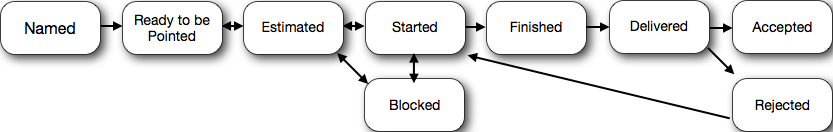
\includegraphics[width=6.25in]{pivotal_images/story_card_workflow}
\caption{Pivotal Kernel Extension Workflow Story Card Alpha}
\label{KernelExtensionWorkflow}
\end{figure*}

\begin{figure*}[ht]
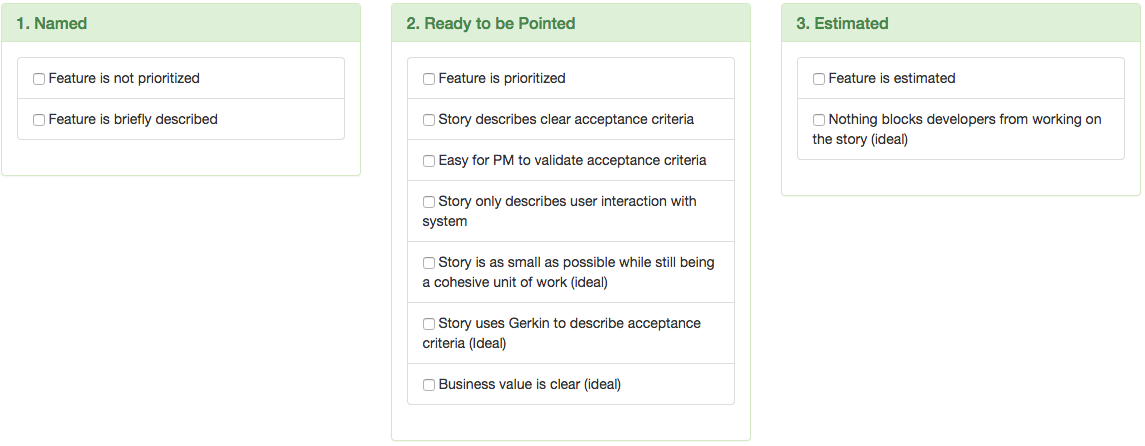
\includegraphics[width=6.25in]{pivotal_images/story_card_prescriptive1}
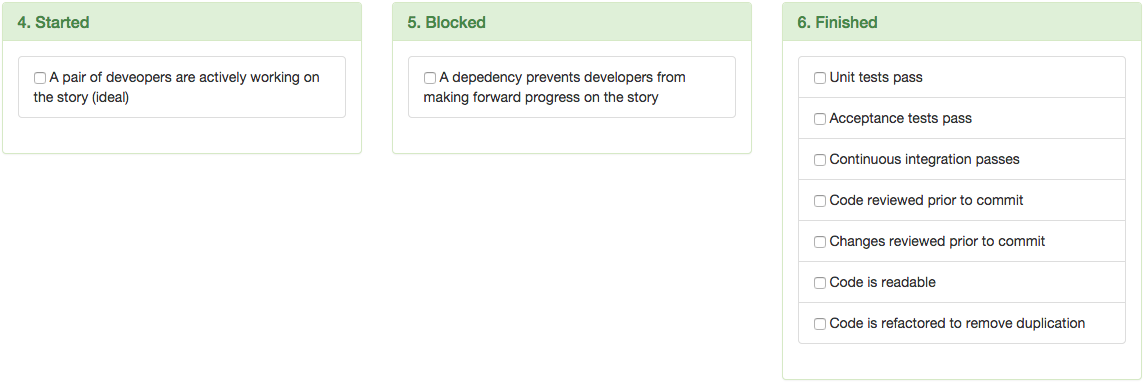
\includegraphics[width=6.25in]{pivotal_images/story_card_prescriptive2}
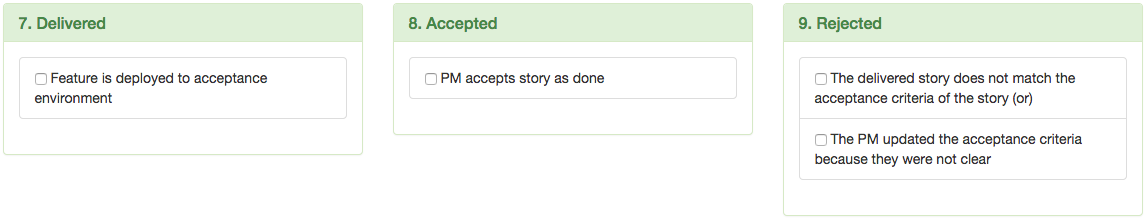
\includegraphics[width=6.25in]{pivotal_images/story_card_prescriptive3}
\caption{Pivotal Kernel Extension for Story Card Alpha}
\label{KernelExtensionPrescriptive}
\end{figure*}


\begin{figure*}[ht]
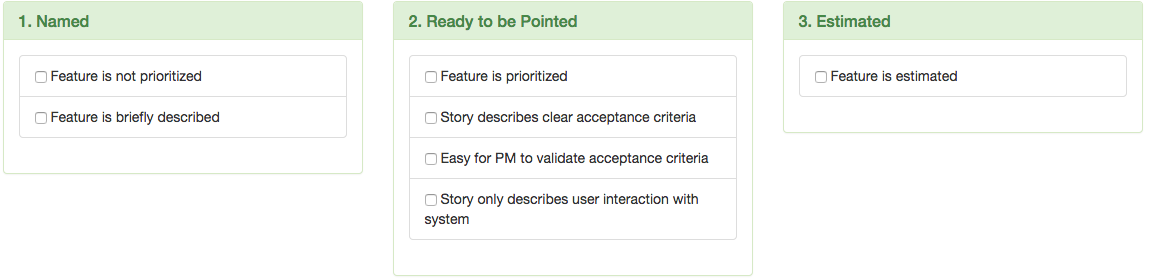
\includegraphics[width=6.25in]{pivotal_images/story_card_descriptive1}
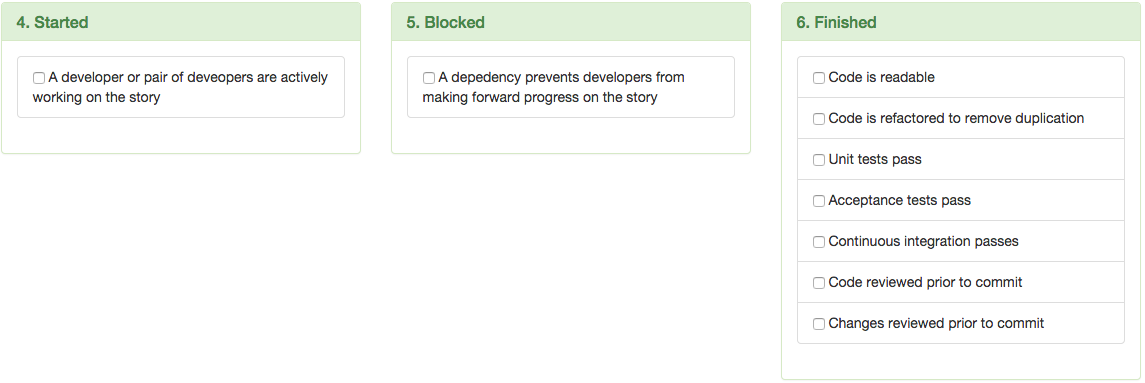
\includegraphics[width=6.25in]{pivotal_images/story_card_descriptive2}
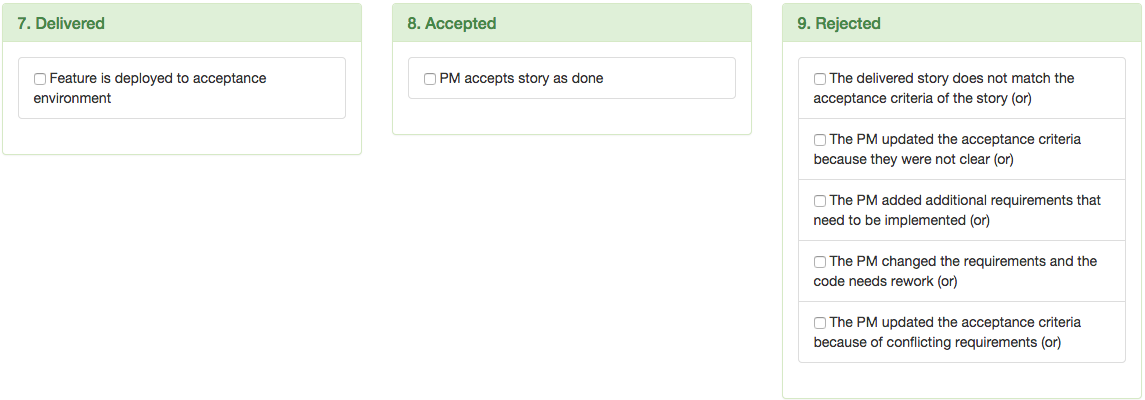
\includegraphics[width=6.25in]{pivotal_images/story_card_descriptive3}
\caption{Pivotal Kernel Extension for Story Card Alpha}
\label{KernelExtensionDescriptive}
\end{figure*}
\section{Discussion}

\subsection{Evaluation of Results and Implications}

The proposed kernel extension corresponds to the story card states in Pivotal Tracker. At first this was not intentional, but frequent tracking of the progress of the story from start to deployment lead to significant similarities between the kernel and the Pivotal Tracker story card states. At one point, one of the researchers was worried about this, that perhaps Pivotal Tracker had too much undue influence on the kernel extension, however, since Pivotal Tracker was modeled to reflect the company's way of working, it should not surprise us that the kernel extension has many similar properties. 

Many of the differences between the prescribed and described kernel extensions can be explained by optional fields or optional interactions in Pivotal Tracker.

When this extension was being reviewed by a co-worker, the engineer objected that the reasons the PM were rejecting stories did not fit our agreed-upon workflow. It became apparent that I needed to separate out a descriptive from a prescriptive mode. There is a shared understanding of how the work should be done, but in practice unusual circumstances cause us to tailor the process to the situation.


\subsection{Threats to Validity}

External Validity. Generalizability across situations: The work done here analyzed software projects at the Silicon Valley office of Pivotal following Extreme Programming. The extension might not be applicable to other teams in industry following Extreme Programming. Replicating the results with other teams would mitigate this threat. Also, the teams following other iterative software development teams may or may not find value. Replicating this with teams following Scrum would mitigate this threat.

Internal Validity. Researcher bias: by using the participant-observer technique its possible that the researcher lost perspective and became biased by being a member of the team. Its possible that a purely outside observer would see something the researcher missed. We used interviews and explicit reviews of the kernel to help mitigate this risk.

\subsection{Inferences}

The two kernel extensions surface whether the Essence Kernel should be prescriptive or descriptive.

The Essence Kernel authors claim that it is a prescriptive model. This makes validating the essence kernel with empirical data challenging, as empirical data would want to create a descriptive model that accurately describes what happens on software projects. While the kernel is meant to be universal, the alphas lack a maintenance states common to many software projects.

\section{Conclusions and Future Work}
\subsection{Summary}
\subsection{Impact}
\subsection{Future Work}

Pivotal has 12 offices around the world. The proposed kernel extension can be validated at other offices.

%% References
%%
%% Following citation commands can be used in the body text:
%% Usage of \cite is as follows:
%%   \cite{key}         ==>>  [#]
%%   \cite[chap. 2]{key} ==>> [#, chap. 2]
%%

%% References with bibTeX database:

\bibliographystyle{elsarticle-num}
% \bibliographystyle{elsarticle-harv}
% \bibliographystyle{elsarticle-num-names}
% \bibliographystyle{model1a-num-names}
% \bibliographystyle{model1b-num-names}
% \bibliographystyle{model1c-num-names}
% \bibliographystyle{model1-num-names}
% \bibliographystyle{model2-names}
% \bibliographystyle{model3a-num-names}
% \bibliographystyle{model3-num-names}
% \bibliographystyle{model4-names}
% \bibliographystyle{model5-names}
% \bibliographystyle{model6-num-names}

\bibliography{bibliography}


\end{document}

%%
%% End of file `elsarticle-template-num.tex'.
